\documentclass[conference]{IEEEtran}

\usepackage{cite}
\usepackage{graphicx}
\usepackage{booktabs}
\usepackage{url}
\usepackage{amsmath}
\usepackage{microtype}

\title{Software Defect Prediction in PROP-1: Comparing Decision Tree, K-Nearest Neighbors, and XGBoost}

\author{\IEEEauthorblockN{Aditya Dubey}}

\begin{document}
\maketitle

\begin{abstract}
Software defect prediction can help rank modules for review, but class imbalance and repeated software-metric patterns can inflate evaluation results if related records occur in both training and test partitions. This paper compares a class-balanced Decision Tree, five-nearest-neighbor (KNN), and XGBoost on PROP-1 from the DefectData repository. The data contain 18,471 observations and 20 numeric CKJM metrics; a module is labeled defective when its bug count is greater than zero. We used the first fold of a shuffled, stratified five-fold group split, grouping identical feature vectors so they cannot cross partitions. On the 3,611-row test fold, XGBoost achieved the highest ROC-AUC (0.819) and top-decile lift (3.33), capturing 189 of 566 defects in the 362 highest-risk modules. The Decision Tree had the highest default-threshold recall (78.1%), while KNN had the highest model accuracy (84.0%), still slightly below the 84.3% all-non-defective baseline. Results are descriptive for this grouped holdout and do not establish statistical superiority.
\end{abstract}

\begin{IEEEkeywords}
software defect prediction, PROP-1, XGBoost, decision tree, K-nearest neighbors, group validation, ROC-AUC, lift
\end{IEEEkeywords}

\section{Introduction}
Software metrics such as size, coupling, and complexity can be used to estimate which software modules are likely to contain defects. This is a binary classification task, but the target is imbalanced: most PROP-1 observations are non-defective. Accuracy alone can therefore obscure how many defects a classifier finds.

The DefectData repository includes PROP-1 in its PROMISE CK dataset collection and reports 18,471 modules, 2,738 defective modules, and 20 predictors \cite{defectdata}. This study compares a Decision Tree, KNN, and XGBoost using confusion matrices, precision, recall, F1, ROC-AUC, and risk-ranked inspection lift. Because repeated feature vectors are common, identical vectors are grouped into the same partition to reduce train/test leakage.

\textbf{Research question:} How effectively do the three classifiers identify defective PROP-1 modules, and which model provides the most useful risk ranking for prioritizing review?

\section{Dataset and Preparation}
The PROP-1 CSV was obtained from the DefectData repository \cite{defectdata,loader}. The source has 18,471 rows, an identifier-like \texttt{Name} field, a \texttt{version} field, 20 numeric software metrics, and the numeric \texttt{bug} count. In accordance with the repository loader, the positive label is defined as \texttt{bug} $>0$ \cite{loader}. The \texttt{Name} and \texttt{version} fields were excluded from predictors.

\begin{table}[t]
\caption{PROP-1 Data Summary}
\label{tab:data}
\centering
\footnotesize
\begin{tabular}{lr}
\toprule
\textbf{Quantity} & \textbf{Value}\\
\midrule
Observations / metrics & 18,471 / 20\\
Defective / non-defective & 2,738 / 15,733\\
Defect prevalence & 14.82\%\\
Missing metric values & 0\\
Exact repeated rows & 3,337\\
Unique feature vectors & 8,672\\
Feature vectors with mixed labels & 661\\
Train / test observations & 14,860 / 3,611\\
Test defects / non-defects & 566 / 3,045\\
\bottomrule
\end{tabular}
\end{table}

Exact repeated rows and repeated metric vectors were retained because the CSV has no unique module identifier to determine whether repetitions are data errors or separate observations with identical measurements. To prevent identical feature vectors from appearing on both sides of the evaluation, we used the first fold of a shuffled, stratified five-fold group split. The resulting test fold contains 3,611 rows (19.6\% of observations) and 566 defects (15.7\% prevalence). No feature values were missing.

\subsection{Descriptive Statistics and Correlation}
The \texttt{loc} metric is strongly right-skewed: mean 206.63, median 73, standard deviation 420.07, variance 176,461.30, skewness 6.11, and excess kurtosis 56.57. This indicates a long upper tail in module size.

Pearson correlations are 0.622 between \texttt{loc} and \texttt{wmc}, and 0.796 between \texttt{max\_cc} and \texttt{avg\_cc}. The Spearman correlation for \texttt{max\_cc} and \texttt{avg\_cc} is 0.934. These statistics describe association, not causation. Correlated metrics can also share model importance.

\section{Methods}
\subsection{Decision Tree}
The Decision Tree recursively partitions the metric space into groups with more homogeneous labels. We used Gini impurity, maximum depth 6, minimum leaf size 10, and balanced class weights. The fitted tree reached depth 6 and had 48 leaves. Balanced class weights raise the training contribution of the minority class \cite{sklearn_tree}.

\subsection{K-Nearest Neighbors}
KNN assigns each test observation the majority label among its five nearest training observations under Euclidean distance. The pipeline applies median imputation and standard scaling before computing distances. We used uniform neighbor weights and $k=5$ \cite{sklearn_knn}.

\subsection{XGBoost}
XGBoost combines sequentially fitted, regularized decision trees \cite{xgboost}. The classifier used 300 estimators, maximum depth 4, learning rate 0.05, row and feature subsampling of 0.8, and L2 regularization of 1. The positive-class weight was set to the training ratio of non-defective to defective observations, $12688/2172 \approx 5.842$. Settings were fixed before test scoring; no hyperparameter search was conducted.

\subsection{Evaluation}
Accuracy, defective-class precision, recall, and F1 are reported at the default 0.5 probability threshold. ROC-AUC summarizes ranking across thresholds, with 0.5 indicating random ranking \cite{fawcett}. For inspection lift, observations are ranked by predicted risk and the defect rate among the top 10\% is divided by the full test-fold defect rate. The top decile contains $\lceil0.10\times3611\rceil=362$ observations. The all-non-defective classifier is included as an accuracy baseline.

\section{Results}
\subsection{Overall Performance}
Table~\ref{tab:metrics} summarizes held-out results. XGBoost achieved the highest ROC-AUC (0.819), F1 (0.478), and top-decile lift (3.33). The Decision Tree had the highest default-threshold recall (78.1\%). KNN had the highest accuracy among the learned models (84.0\%), but remained below the 84.3\% accuracy of the all-non-defective baseline.

\begin{table*}[t]
\caption{Performance on the Grouped PROP-1 Test Fold}
\label{tab:metrics}
\centering
\footnotesize
\begin{tabular}{lrrrrrr}
\toprule
\textbf{Model} & \textbf{Accuracy} & \textbf{Precision} & \textbf{Recall} & \textbf{F1} & \textbf{ROC-AUC} & \textbf{Top-Decile Lift}\\
\midrule
Decision Tree & 62.7\% & 26.5\% & \textbf{78.1\%} & 0.396 & 0.778 & 2.93\\
KNN ($k=5$) & \textbf{84.0\%} & \textbf{48.6\%} & 32.7\% & 0.391 & 0.745 & 3.15\\
XGBoost & 75.0\% & 35.5\% & 72.8\% & \textbf{0.478} & \textbf{0.819} & \textbf{3.33}\\
Majority baseline & 84.3\% & -- & 0.0\% & 0.000 & -- & 1.00\\
\bottomrule
\end{tabular}
\end{table*}

\subsection{Confusion Matrices}
Table~\ref{tab:confusion} reports true-positive/false-negative and false-positive/true-negative counts. XGBoost identified 412 defects and missed 154; the Decision Tree identified 442 defects and missed 124. KNN produced fewer false alarms but missed 381 of the 566 test defects.

\begin{table}[t]
\caption{Confusion Counts (TP/FN, FP/TN)}
\label{tab:confusion}
\centering
\footnotesize
\begin{tabular}{lrr}
\toprule
\textbf{Model} & \textbf{TP / FN} & \textbf{FP / TN}\\
\midrule
Decision Tree & 442 / 124 & 1,224 / 1,821\\
KNN ($k=5$) & 185 / 381 & 196 / 2,849\\
XGBoost & 412 / 154 & 747 / 2,298\\
\bottomrule
\end{tabular}
\end{table}

\subsection{ROC and Risk-Ranked Inspection}
Fig.~\ref{fig:roc} shows ROC curves. All three models rank better than random, and XGBoost has the highest AUC. The difference is descriptive for this fold and is not tested for statistical significance.

In the top 10\% of ranked observations (362 rows), XGBoost captured 189 of 566 defects (33.4\% of test defects) for 3.33$\times$ lift. KNN captured 179 (31.6\%; 3.15$\times$ lift), and the Decision Tree captured 166 (29.3\%; 2.93$\times$ lift). Fig.~\ref{fig:gains} plots cumulative gains as review capacity increases.

\begin{figure*}[t]
\centering
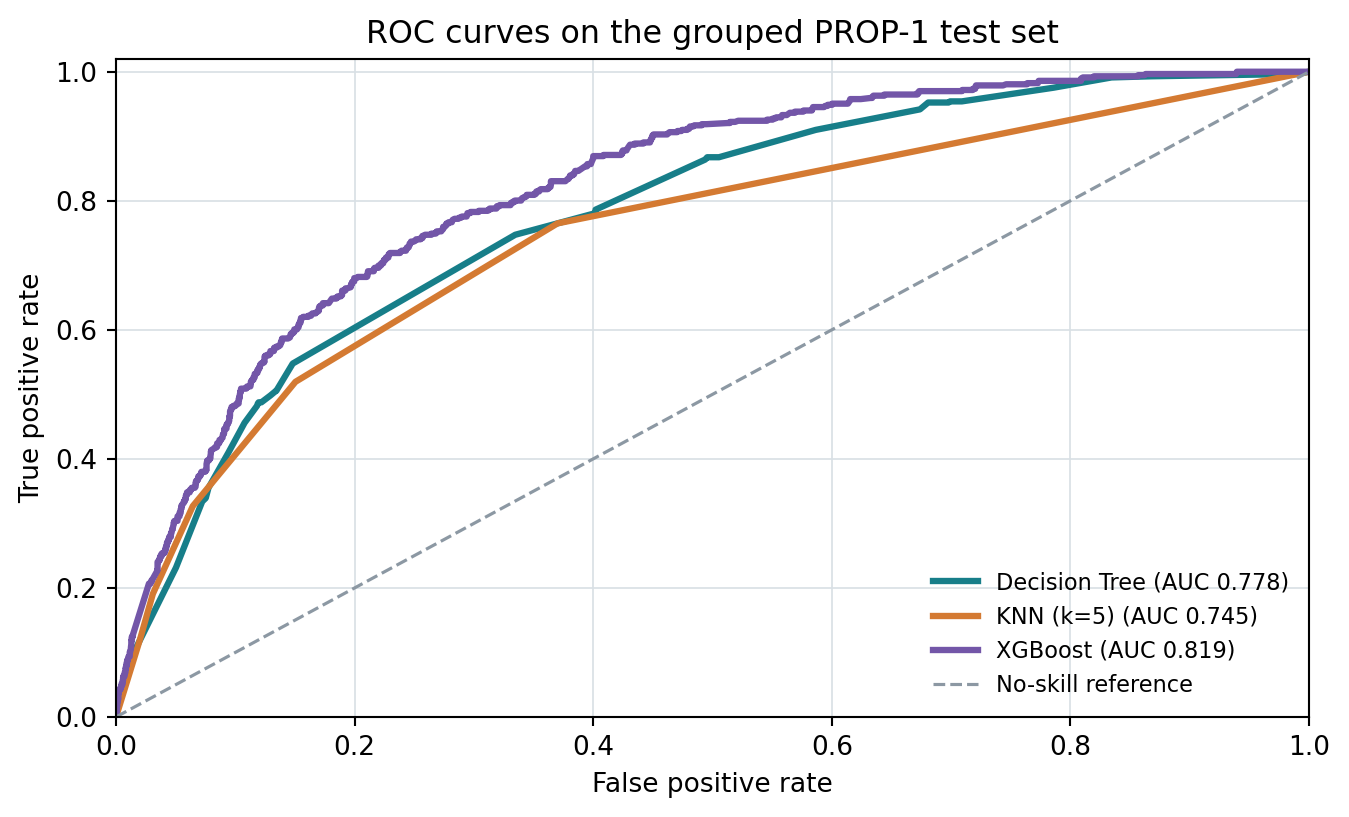
\includegraphics[width=0.78\textwidth]{figures/roc_curve.png}
\caption{ROC curves on the grouped PROP-1 test fold.}
\label{fig:roc}
\end{figure*}

\begin{figure*}[t]
\centering
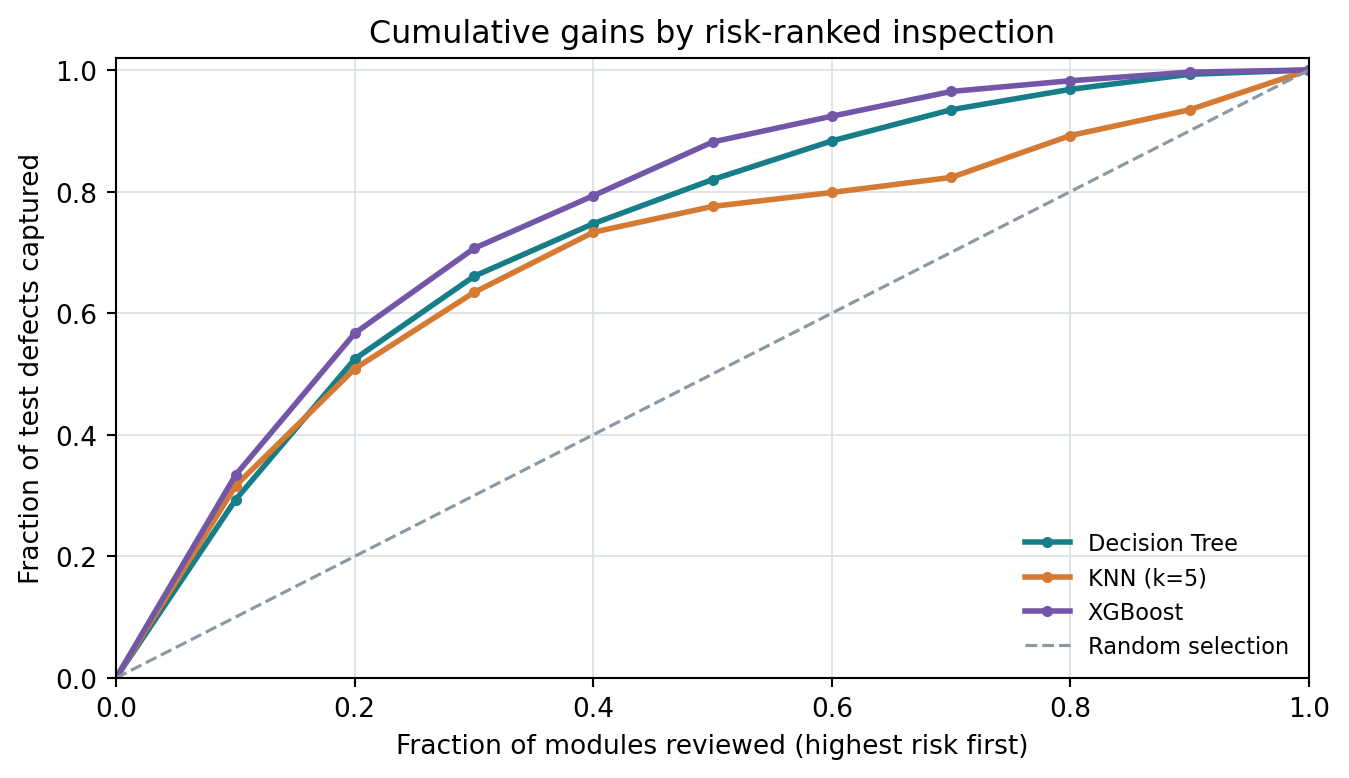
\includegraphics[width=0.78\textwidth]{figures/cumulative_gains.png}
\caption{Cumulative fraction of test-fold defects captured by reviewing observations in descending predicted-risk order.}
\label{fig:gains}
\end{figure*}

\subsection{Feature Importance}
XGBoost's five largest gain-based importance values were \texttt{ce} (0.156), \texttt{cbo} (0.111), \texttt{cam} (0.083), \texttt{npm} (0.054), and \texttt{loc} (0.046). These are model-specific split summaries, not causal effects. Correlated features can share importance.

% Flush result figures and tables before discussion, conclusion, and references.
\clearpage

\section{Discussion}
The grouped split prevents identical metric vectors from leaking across partitions, but it also creates a harder evaluation than a row-wise random split. The prevalence in the test fold (15.7\%) is close to the full-data rate (14.8\%). The number of repeated feature patterns and the 661 patterns associated with both labels suggest that these metrics do not uniquely determine defect status.

XGBoost offers the strongest overall risk ranking by ROC-AUC, F1, and top-decile lift. The Decision Tree finds slightly more defects at the default threshold, while KNN makes the fewest false-positive predictions. All models have a precision/recall trade-off and fall short of the majority-class baseline on accuracy. Model selection should therefore depend on review capacity and the relative cost of missed defects and false alarms.

\subsection{Limitations and Statistical Significance}
Only PROP-1 and one grouped holdout fold were analyzed. No cross-validation summary, hyperparameter tuning, external validation, or hypothesis test was performed; no p-value or statistical superiority claim is made. Results may vary with the group partition and may not transfer to other projects. Repeated patterns and mixed labels limit predictability. Feature importance and correlations are not causal evidence.

\section{Conclusion}
On the grouped PROP-1 holdout, XGBoost achieved the strongest ranking performance (ROC-AUC 0.819; top-decile lift 3.33) and highest F1 (0.478). The Decision Tree had the highest default-threshold recall (78.1\%), while KNN had the highest accuracy among learned models but did not exceed the majority-class baseline. These results support XGBoost as the most useful risk ranker among the tested configurations, with validation across additional grouped folds needed before making a broader claim.

\section*{Reproducibility}
The analysis used scikit-learn 1.7.2 and XGBoost 3.4.1. Group identities were formed from identical 20-metric feature vectors; the first split from \texttt{StratifiedGroupKFold(n\_splits=5, shuffle=True, random\_state=42)} was evaluated. The source label is \texttt{bug > 0}; \texttt{Name} and \texttt{version} were excluded from model inputs.

\bibliographystyle{IEEEtran}
\bibliography{references}

\end{document}
